In this task the objective is to design a linear quadratic regulator [LQR] able to follow the smooth optimal trajectory generated in the 
previous task.

\section{Problem setup}
The first step needed to achieve our goal is to linearize the system dynamics, computed in Task 0, about the smooth optimal trajectory $(x^{opt},u^{opt})$,
obtained in Task 2, in order to obtain $A^{opt}$ and $B^{opt}$. Then the idea is to use a regulator that will reject disturbances, and will try to follow the 
optimal trajectory. To do that, we have to solve a Linear quadratic optimization problem, with a quadratic cost function, in which the cost matrices were a degree of freedom,
and the linearized dynamics over the optimal trajectory.

\section{Parameters and results}
Running some simulation, we found great results using as matrices $Q^{reg}$ and $R^{reg}$ the same matrices used in the cost function for the Newton's method.
To test the performances of our regulator, we will inject in the system some random error (5-10-20\% of the maximum value reached during the trajectory for each state)
in the initial conditions.
\\Then we need to solve the LQ optimal control problem to find the feedback gain matrix $K_t^{reg}$ needed to update $u$ bye the equation: 
\begin{center}
    $u_t=u_t^{opt}+K_t^{reg}(x_t-x_t^{opt})$\\
    $x_{t+1}=f_t(x_t,u_t)$
\end{center}

In the following plots we can see the tracking performances of the LQR algorithm used.
\begin{figure}[!h]
    \center
	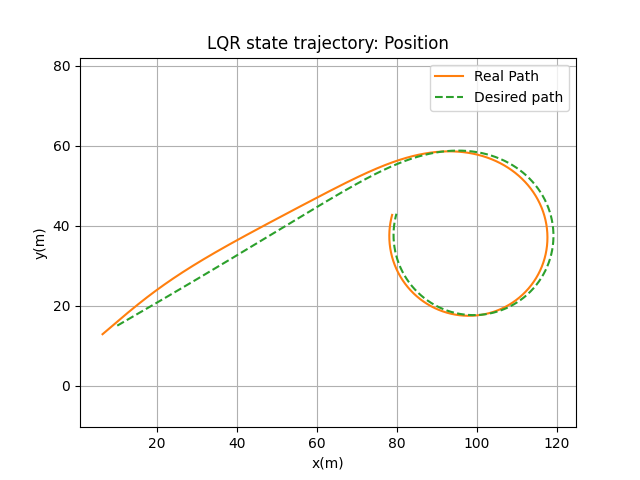
\includegraphics[height=70mm]{figs/_lqr_xy_5.png}	
	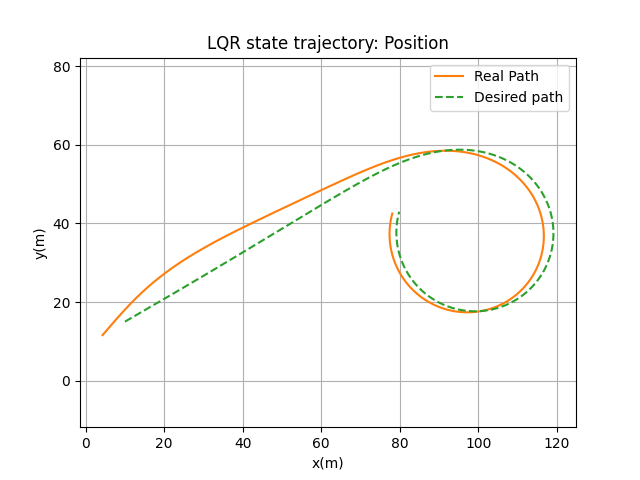
\includegraphics[height=70mm]{figs/_lqr_xy_10.png}	
    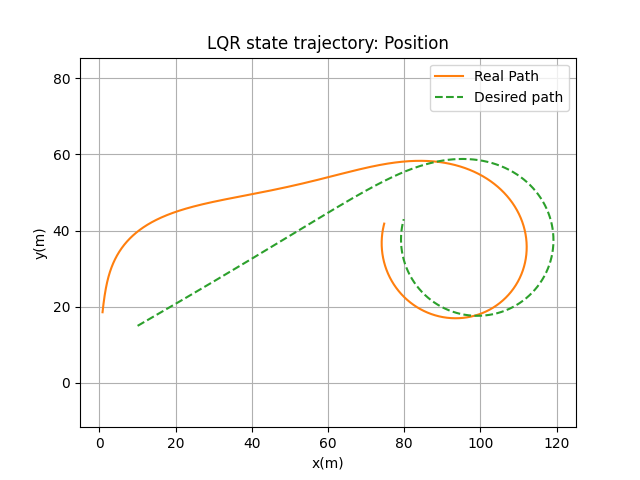
\includegraphics[height=70mm]{figs/_lqr_xy_20.png}	
	\caption{Tracked position trajectory with 5-10-20\% relative error on $x_0$}
\end{figure} 

\begin{figure}[!h]
    \center
	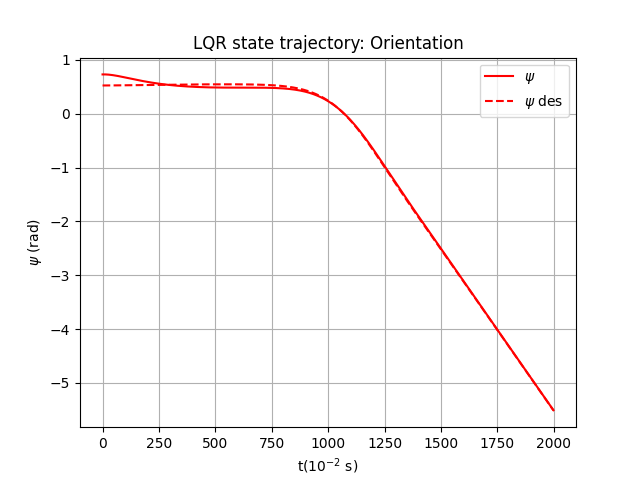
\includegraphics[height=70mm]{figs/_lqr_psi_5.png}	
	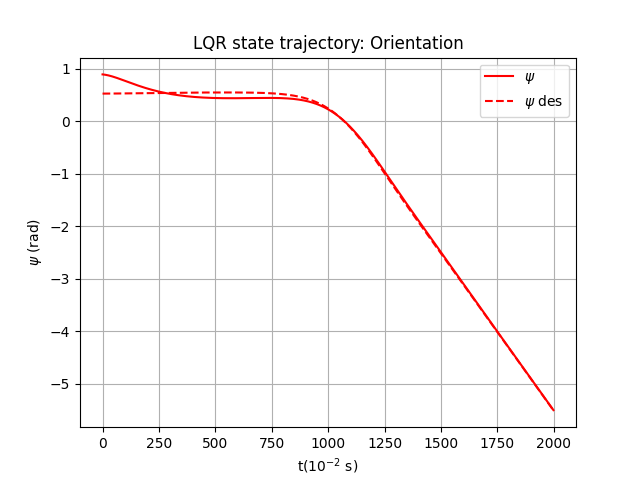
\includegraphics[height=70mm]{figs/_lqr_psi_10.png}	
    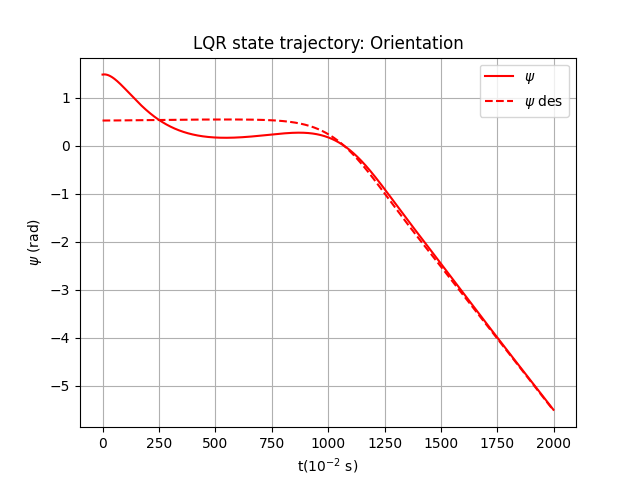
\includegraphics[height=70mm]{figs/_lqr_psi_20.png}	
	\caption{Tracked $\psi$ trajectory with 5-10-20\% relative error on $x_0$}
\end{figure} 

\begin{figure}[!h]
    \center
	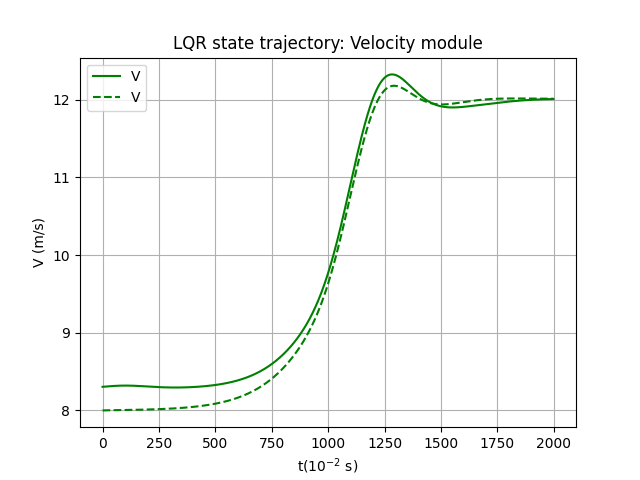
\includegraphics[height=70mm]{figs/_lqr_V_5.png}	
	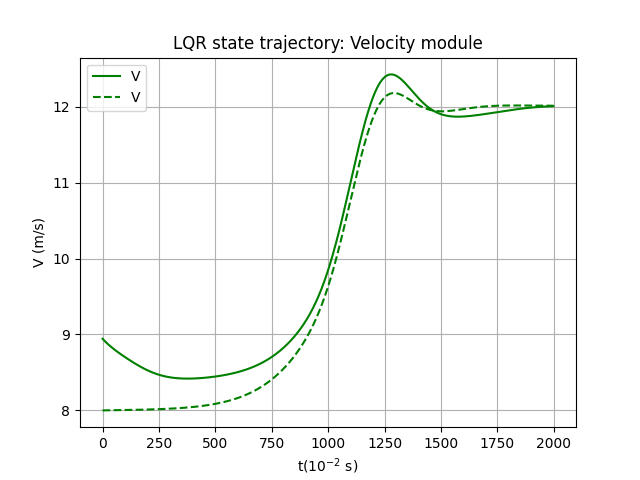
\includegraphics[height=70mm]{figs/_lqr_V_10.png}	
    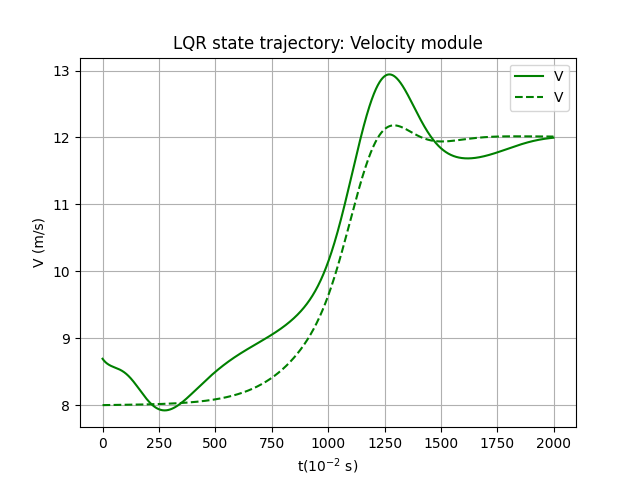
\includegraphics[height=70mm]{figs/_lqr_V_20.png}	
	\caption{Tracked $V$ trajectory with 5-10-20\% relative error on $x_0$}
\end{figure} 

\begin{figure}[!h]
    \center
	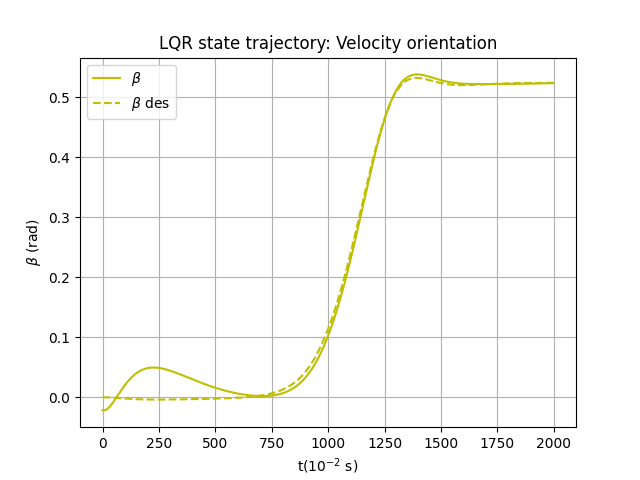
\includegraphics[height=70mm]{figs/_lqr_beta_5.png}	
	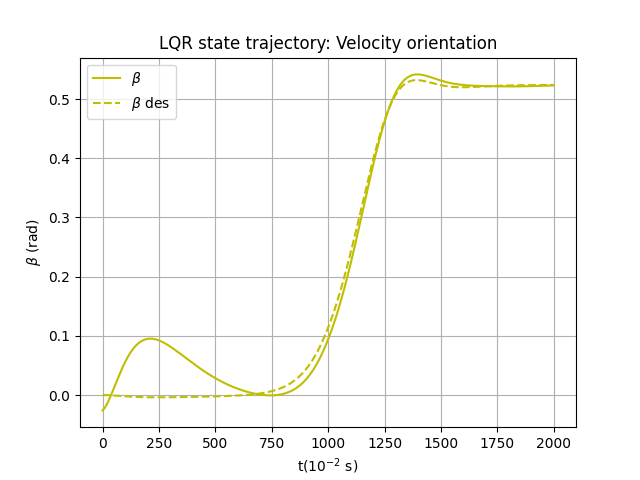
\includegraphics[height=70mm]{figs/_lqr_beta_10.png}	
    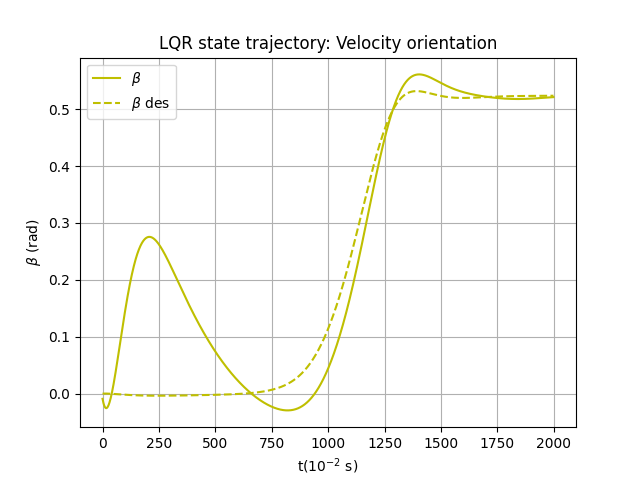
\includegraphics[height=70mm]{figs/_lqr_beta_20.png}	
	\caption{Tracked $\beta$ trajectory with 5-10-20\% relative error on $x_0$}
\end{figure} 

\begin{figure}[!h]
    \center
	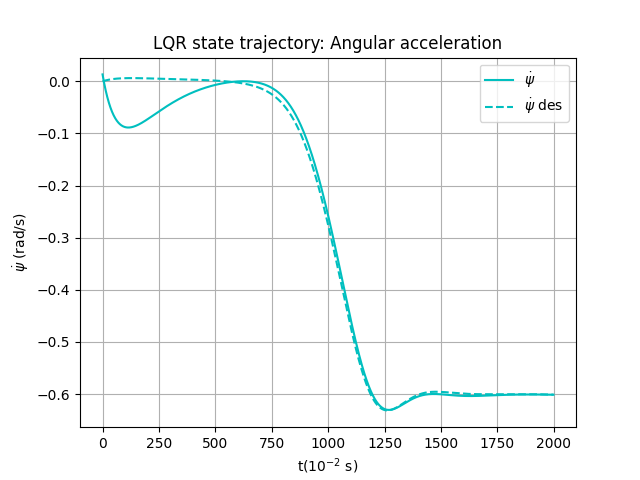
\includegraphics[height=70mm]{figs/_lqr_psidot_5.png}	
	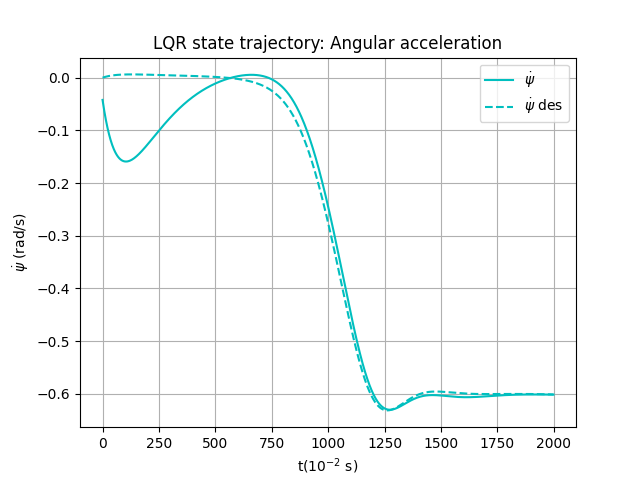
\includegraphics[height=70mm]{figs/_lqr_psidot_10.png}	
    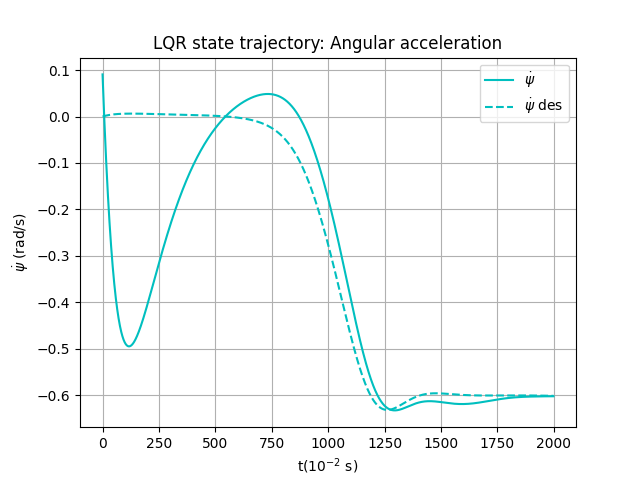
\includegraphics[height=70mm]{figs/_lqr_psidot_20.png}	
	\caption{Tracked $\dot{\psi}$ trajectory with 5-10-20\% relative error on $x_0$}
\end{figure} 

\begin{figure}[!h]
    \center
	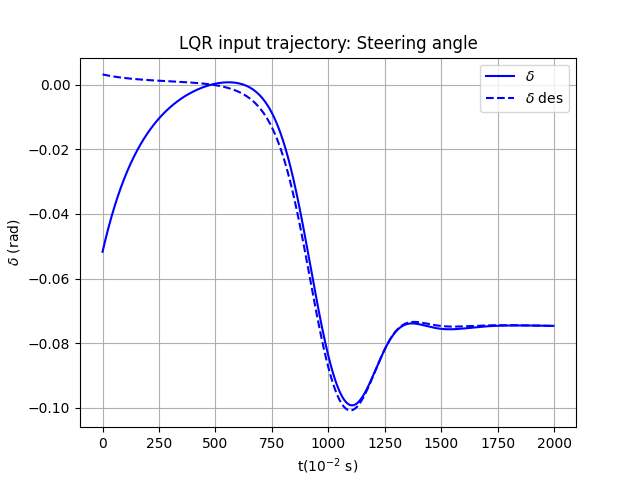
\includegraphics[height=70mm]{figs/_lqr_delta_5.png}	
	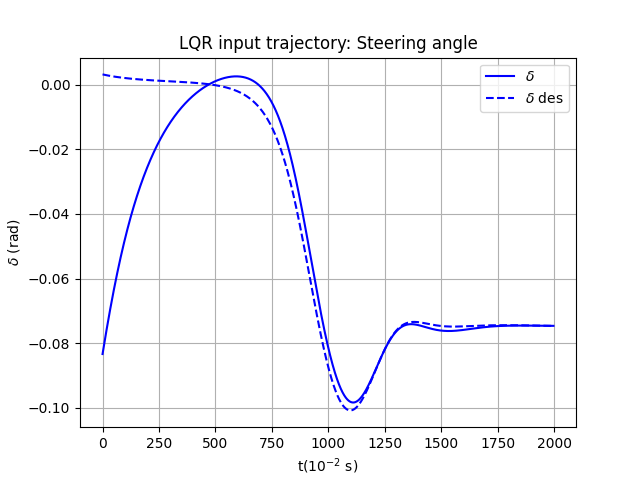
\includegraphics[height=70mm]{figs/_lqr_delta_10.png}	
    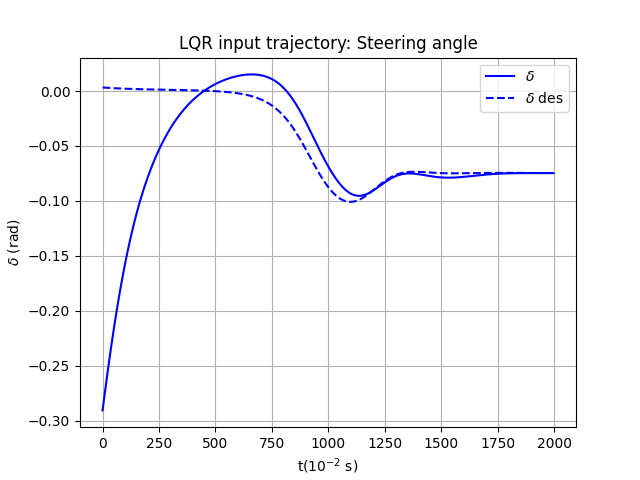
\includegraphics[height=70mm]{figs/_lqr_delta_20.png}	
	\caption{Tracked $\delta$ trajectory with 5-10-20\% relative error on $x_0$}
\end{figure} 

\begin{figure}[!h]
    \center
	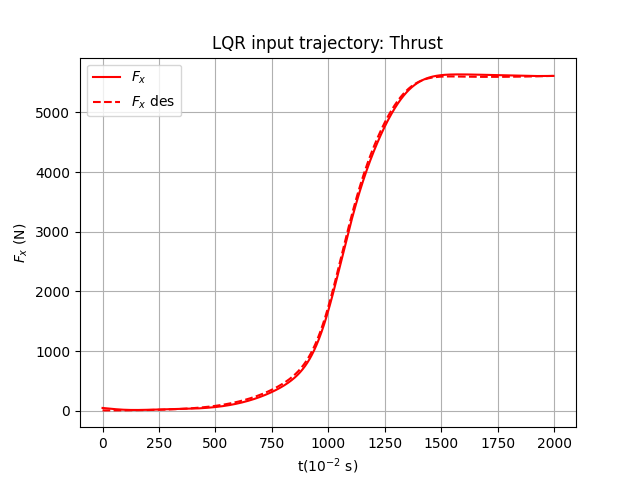
\includegraphics[height=70mm]{figs/_lqr_Fx_5.png}	
	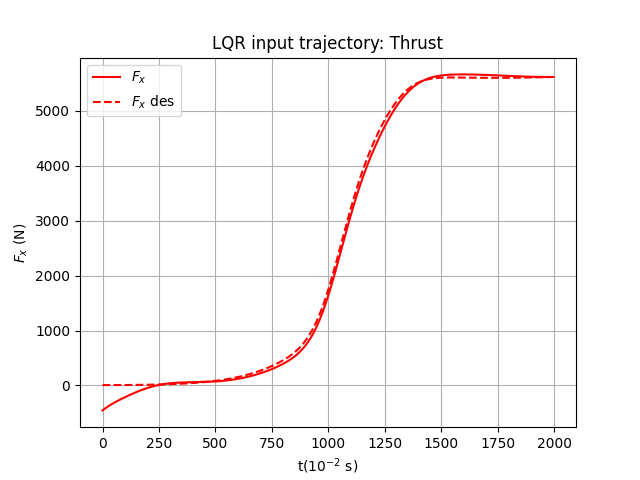
\includegraphics[height=70mm]{figs/_lqr_Fx_10.png}	
    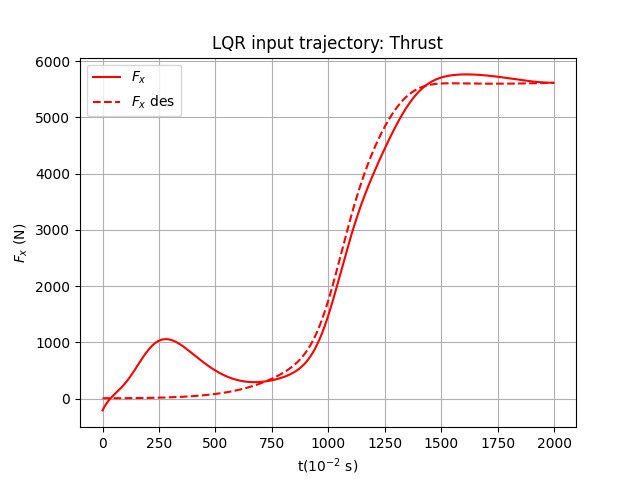
\includegraphics[height=70mm]{figs/_lqr_Fx_20.png}	
	\caption{Tracked $F_x$ trajectory with 5-10-20\% relative error on $x_0$}
\end{figure} 

\FloatBarrier
\section{Conclusions}
The LQR algorithm proved to be very robust with respect to initial condition error, 
indeed all the state variables with 5\% and 10\% error were accurately tracked and
only the trajectory with 20\% error reached the desired velocity bringing the system
in a steady state with some offset in the final position. 